\documentclass[a4paper, 10pt]{article}%тип документа

%Русский язык
\usepackage[T2A]{fontenc} %кодировка
\usepackage[utf8]{inputenc} %кодировка исходного кода
\usepackage[english,russian]{babel} %локализация и переносы

%Вставка картинок
\usepackage{graphicx}
\graphicspath{{pictures/}}
\DeclareGraphicsExtensions{.pdf,.png,.jpg}

%Графики
\usepackage{pgfplots}
\pgfplotsset{compat=1.9}

%Математика
\usepackage{amsmath, amsfonts, amssymb, amsthm, mathtools}

%Заголовок
\author{\textbf{Муляревич Андрей Игоревич}}
\title{Работа 1.1.1 \\
Определение систематических и случайных погрешностей при измерении удельного сопротивления нихромой проволоки}


\begin{document}
\maketitle 
\newpage
В работе используеются: линейка, линейка, штангенциркуль, микрометр, отрезок проволоки из нихрома, амперметр, вольтметр, источник ЭДС, мост постоянного тока, реостат, ключ. 
\begin{enumerate}
\item Точность измерения с помощью штангенциркуля -- 0,05 мм. Точность измерения с помощью микрометра -- 0,01 мм.
\item Измеряем диаметр проволки с помощью штангенциркуля ($d_1$, табл. 1) и микрометра ($d_2$, табл. 2) на 10 различных участках.

При измерении диаметра проволоки штангенциркулем случайная погрешность отсутствует. Следовательно, точность резульата определяется только точностью штангенциркуля $\Rightarrow  d_1 = $ 0.44 $\pm$ 0.05 мм. 

При измерении микрометром есть как систематичская, так и случайная ошибка:
\[ \sigma_{\text{сист}}  = 0,01 \text{ мм, }
\sigma_{\text{сл}}  = \dfrac{1}{N} \cdot \sqrt{\sum_{i = 1}^N (d - \overline{d})^2} = \sqrt{7,45\cdot10^{-4}} \approx 0,027 \text{ мм}\]
\[ \sigma =  \sqrt{\sigma_{\text{сист}}^2 + \sigma_{\text{сл}}^2} \approx 0,027 \text{мм}\]
\[ d_2 = 0,375 \pm 0,027\text{мм}\]
Поскольку погрешность микрометра на порядок меньше погрешности штангенциркуля, для расчета площади поперечного сечения проволоки будем использовать значение, полученное измерением с помощью микрометра.
\item Определим площадь поперечного сечения проволоки: 
\[ S = \dfrac{ \pi d^2 }{4} = \dfrac{3,14 \cdot (0,364)^2}{4} \approx 0,11 \text{ мм}^2\]
Погрешность находим по формуле:
\[ \left( \dfrac{\sigma_{s}}{S} \right)^2 =\dfrac{2 \text{ }\sigma_{d_2}}{d_2} \Rightarrow \dfrac{\sigma_{s}}{S} = \dfrac{\sqrt{2} \text{ } \sigma_{d_2}}{d_2} \Rightarrow \sigma_{s} =\dfrac{\sqrt{2} \text{ } \sigma_{d_2} S}{d_2} \approx 0,011 \text{мм}^2\]
\item см. табл. 2
\item Очевидно, что надо мерять способом показанным на рис. 1a, так как:

для схемы на рисунке 1а: $R_{\text{пр}}$/$R_{\text{V}} = 5 / 400 = 0,0125$

а для схемы на рисунке 1б: $R_{\text{A}}$/$R_{\text{пр}} = 1,2 / 5 = 0,24$
\newpage
\item Собираем схему рис. 1 \\
\begin{figure}[h]
\center{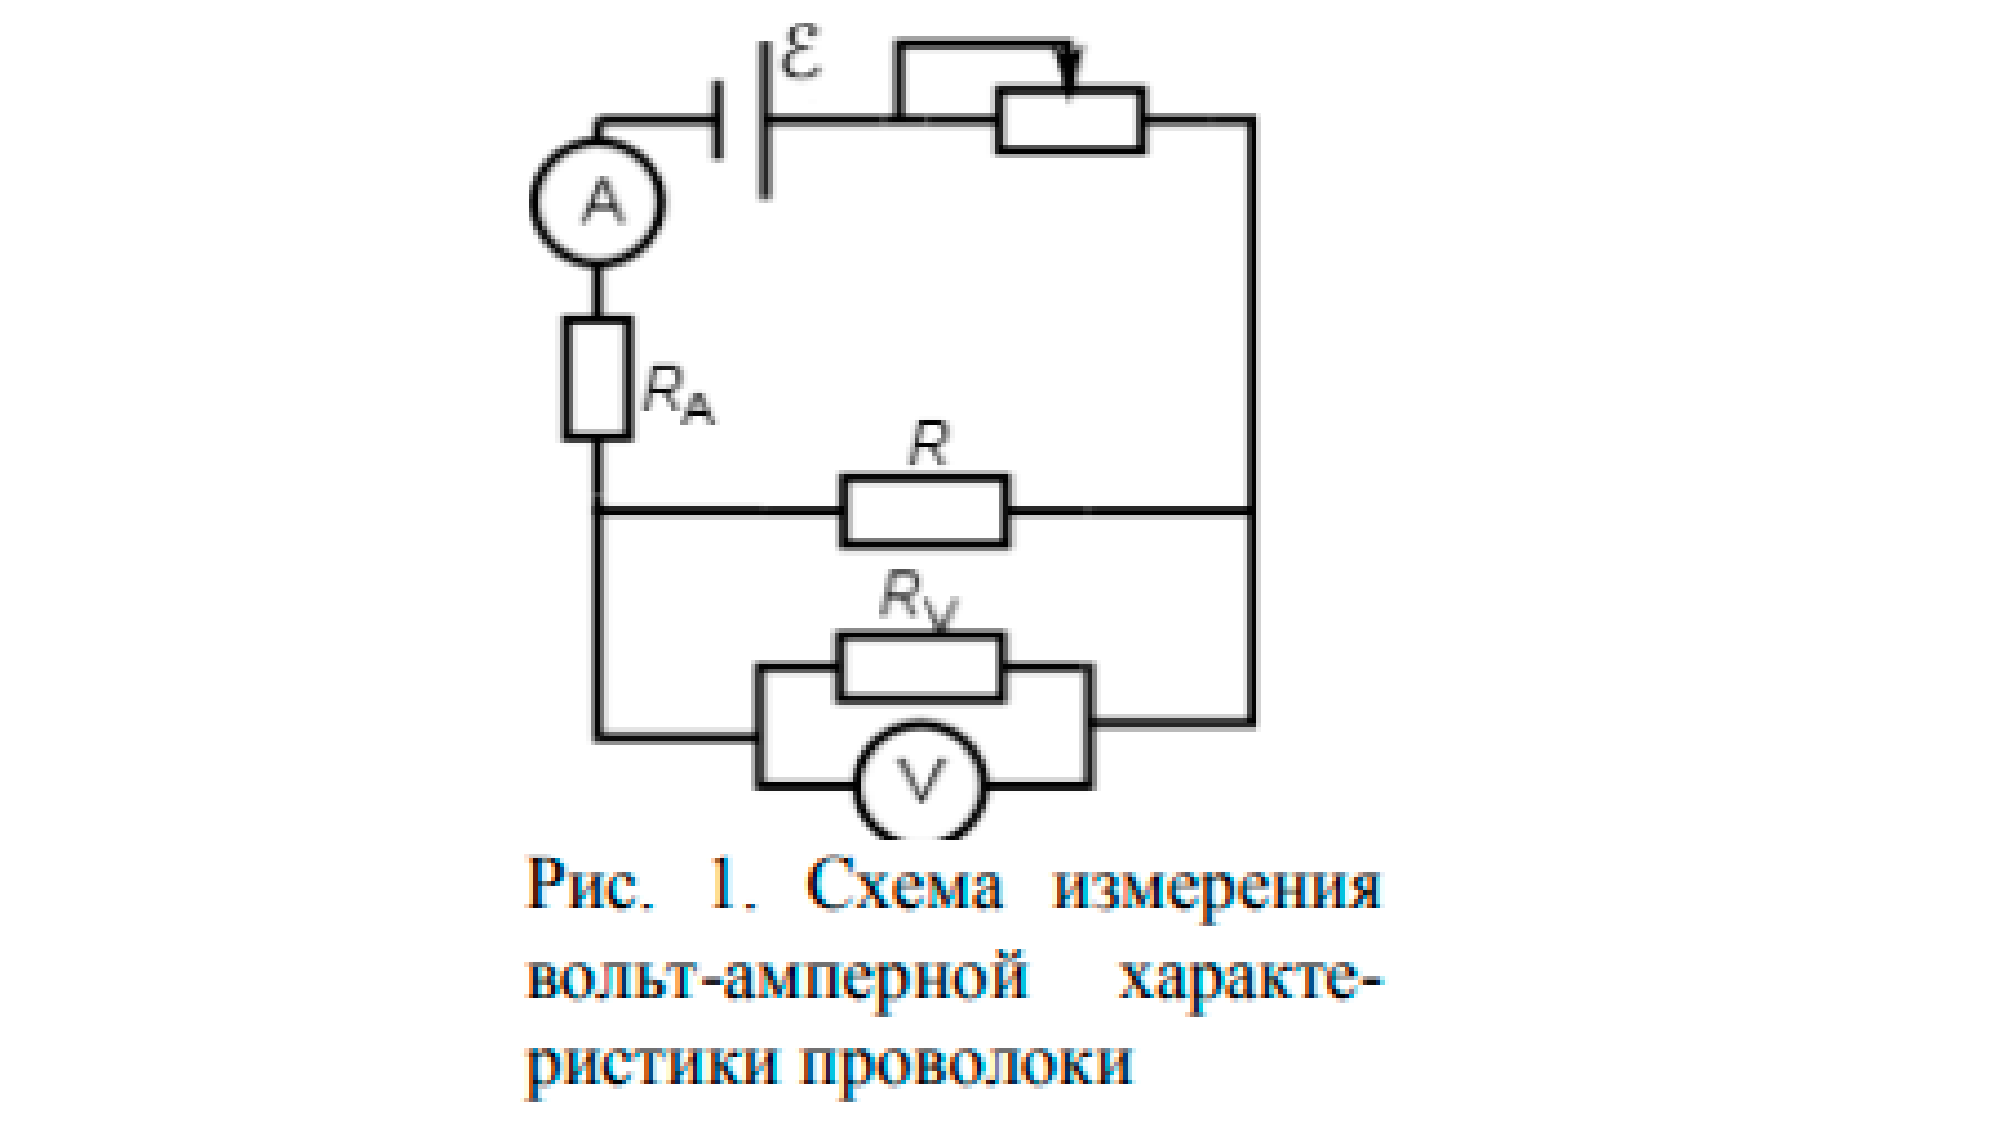
\includegraphics[scale = 0.25]{Laba3shema.pdf}}
\end{figure}
\item Опыт проводим для трех величин: 
$ l_1 = (50\pm 0,1) \text{ см}, l_2 = (30\pm0,1) \text{ см}, l_3 = (10\pm 0,1) \text{ см.}$ \\
Измерения ведем для возрастающих и убывающих значений тока, все измерения записываем в табл. 3, табл. 4, табл. 5.
\item Строим графики зависимостей V = f(I) для всех трех отрезков проволоки, так как 1 прямая не проходит через все точки, но с точность до погрешностей мы ее провести можем, то, ищем график прямой V = f(I) по формуле
\[ V = \dfrac{ \left\langle VI \right\rangle }{ \left\langle I^2 \right\rangle } R_\text{пр} \]
\begin{tikzpicture}
\begin{axis}[ 
		title = $l_1$,
		height = 0.32\paperheight, 
		width = 0.65\paperwidth,
		legend pos = north west,	
		axis x line = bottom,
		axis y line = left,
		ymin = 150, xmin = 30,
		ymax = 570, xmax = 110,
		grid = major,
		xlabel = {$I$, $\text{мА}$},
		ylabel = {$V$, $\text{мВ}$},]
	\addplot+ [smooth,] coordinates
	{
		(31.9, 168) (36.2, 188) (39.3, 204) (45.5, 240) (50.4, 254) 
		(57.9, 304) (73.9, 388) (90.5, 476) (105.8, 548)
	};
	\addplot+ [dashed, smooth,] coordinates
	{
		(105.8, 548) (92.3, 476) (82.6, 432) (73.4, 384) (63.3, 348)
		(54.5, 284) (49.6, 260) (43.4, 228) (38.5, 204)
	};
	\legend {increase, decrease};
\end{axis}
\end{tikzpicture} \\
\begin{tikzpicture}
\begin{axis} [title = $l_2$,
		height = 0.3\paperheight, 
		width = 0.6\paperwidth,
		legend pos = north west,	
		axis x line = bottom,
		axis y line = left,
		grid = major,
		ymin = 100, ymax = 460, 
		xmin = 30, xmax = 145,
		xlabel = {$I$, $\text{мА}$},
		ylabel = {$V$, $\text{мВ}$},
		]
	\addplot+ [smooth] coordinates
	{
		(39.2, 124) (47.4, 148) (59.1, 184) (70.1, 220) (84.0, 264)
		(106.8, 340) (140.5, 440)
	};
	\addplot+[dashed, smooth] coordinates
	{
		(140.5, 440) (110.5, 344) (92.4, 292) (83.4, 260) (65.3, 200)
		(50, 156) (39.2, 120)
	};
	\legend {increase, decrease};
\end{axis}
\end{tikzpicture} \\

\begin{tikzpicture}
\begin{axis} [title = $l_3$,
		height = 0.3\paperheight, 
		width = 0.6\paperwidth,	
		axis x line = bottom,
		legend pos = north west,
		axis y line = left,
		grid = major,
		ymin = 20, ymax = 220, 
		xmin = 30, xmax = 220,
		xlabel = {$I$, $ \text{мА}$},
		ylabel = {$V$, $ \text{мВ}$},]
	\addplot+ [smooth] coordinates
	{
		(41.0, 40) (53.3, 60) (68.3, 72) (88.5, 96) (110.8, 116) 
		(141, 148) (201, 208)
	};
	\addplot+ [dashed, smooth] coordinates
	{
		(201, 208) (133.3, 140) (107.3, 112) (86.4, 92) (66.7, 72)
		(55.3, 56) (42.3, 44)
	};
	\legend {increase, decrease};
\end{axis}
\end{tikzpicture}
\item Запишем в табл. 6 данные средних значений некоторых величин, которые мы в дальнейшем будем использовать.
\item По формулам 
\[ \sigma^{\text{случ}}_{R_{\text{ср}}} = \dfrac{1}{\sqrt{N}}\cdot \sqrt{\dfrac{\left\langle V^2 \right\rangle }{\left\langle I^2 \right\rangle} - R^{2}_{\text{ср}}}\] 
\[ \sigma^{\text{сист}}_{R_{\text{ср}}} = R_{\text{ср}}\sqrt{\left( \dfrac{\sigma_{V}}{\langle V\rangle} \right) ^{2} + \left( \dfrac{\sigma_{I}}{\langle I\rangle} \right) ^{2} } \]
\[ \sigma_R =  \sqrt{\sigma_{\text{сист}}^2 + \sigma_{\text{сл}}^2} \]
\[ R_\text{ср} = \dfrac{\left\langle VI \right\rangle}{\left\langle I^2 \right\rangle}\]
Находим сопротивления и погрешности для каждого из участков проволоки. Данные заносим в табл.7. В эту же таблицу заносим результаты измерения сопротивления мостом Уитстона (P4833), изображенном ниже.
\begin{figure}[h]
\center{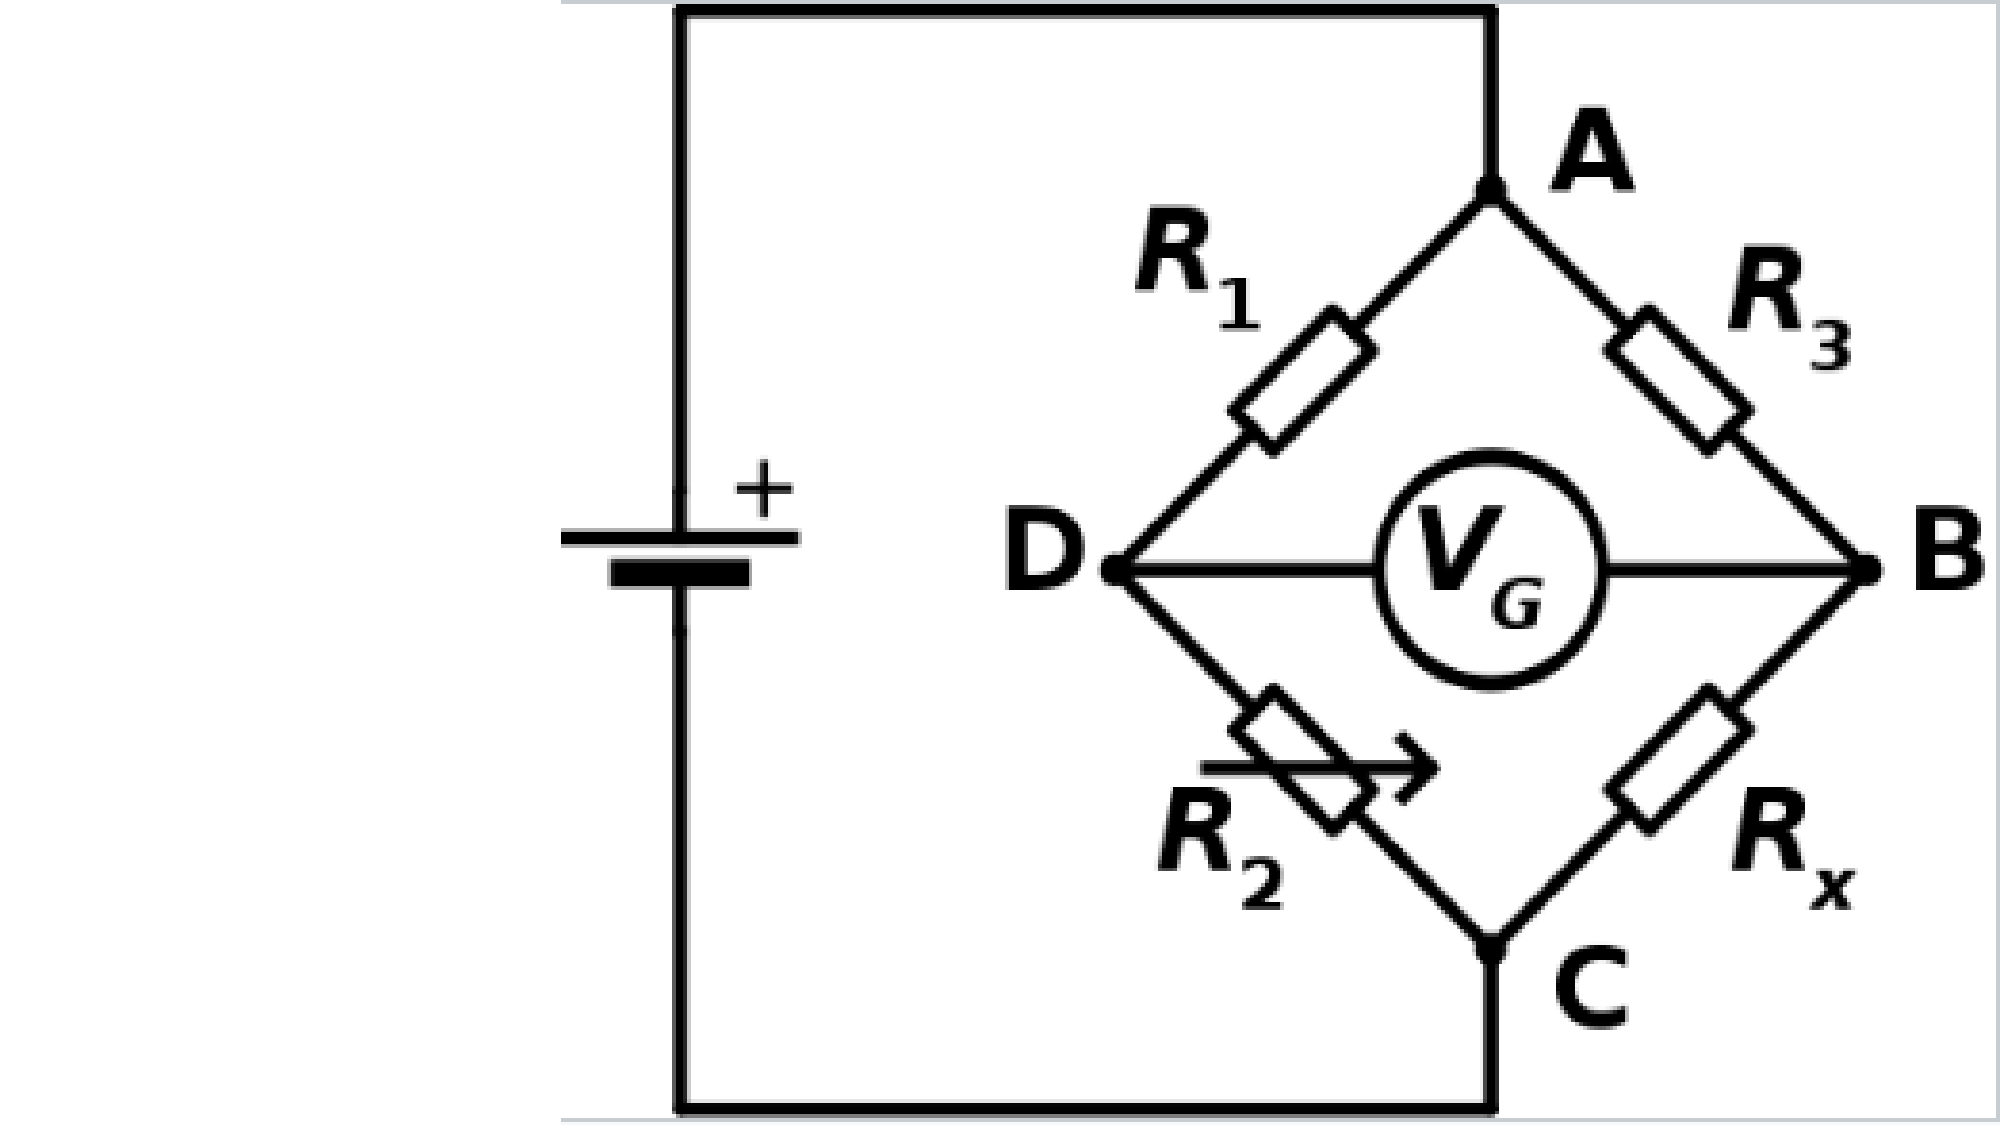
\includegraphics[scale = 0.25]{Laba3shema2.pdf}}
\end{figure}
\item по формулам 
\[ \sigma_{\rho} = \rho \sqrt{\left( \dfrac{\sigma_{R}}{R} \right) ^{2} + \left( \dfrac{\sigma_{l}}{l} \right) ^{2} + \left( \dfrac{\sigma_{S}}{S} \right) ^{2} } \]
\[\rho = \dfrac{R \cdot S}{l}\]
находим удельное сопротивление и погрешность для каждой из длин проволоки и заносим эти значения в табл.8.
\end{enumerate}
Окончательно:$\rho = 1,15 \dfrac{\text{Ом} \cdot \text{мм}^2}{\text{м}}$

Полученное значение удельного сопротивления сравниваем с табличными значениями. В справочнике (Физические велечины. М.: Энергоиздат, 1991. С. 444) для удельного сопротивления нихрома при 20 $ ^\circ C$ в зависимости от массового содержания компонента сплава меняются в промежутке  $1,05 - 1,4\dfrac{\text{Ом} \cdot \text{мм}^2}{\text{м}}$. Полученное значение наиболее близко к значению  $1,16\dfrac{\text{Ом} \cdot \text{мм}^2}{\text{м}}$ для сплава с содержанием 77 процентов Никеля, 20 процентов Хрома, 2 Марганца и 1 Железа(проценты по массе).
\newpage
\begin{table}
	\caption{Результаты измерения диаметра проволоки}
	\begin{tabular}{|r|c|c|c|c|c|c|c|c|c|c|c|}
	\hline
& 1 & 2 & 3 & 4 & 5 & 6 & 7 & 8 & 9 & 10\\
\hline
$d_1$, мм & 0,45 & 0,45 & 0,40 & 0,40 & 0,45 & 0,50 & 0,45 & 0,4 & 0,45 & 0,45 \\
\hline
$d_2$, мм & 0,38 & 0,41 & 0,36 & 0,37 & 0,40 & 0,41 & 0,39 & 0,36 & 0,32 & 0,35 \\
\hline
\multicolumn{1}{|r|}{} & \multicolumn{5}{c}{ \( \overline{d_{1}} =  0,44\) мм}  & \multicolumn{5}{c|}{ \( \overline{d_{2}} = 0,37 мм \) мм}\\
\hline
\end{tabular}
\end{table}

\begin{table}
\caption{Основные характеристики амперметра и вольтметра}
\begin{tabular}{|p{3cm}|p{5cm}|p{5cm}|}
\hline
& Вольтметр & Амперметр \\
\hline
Система & Магнитоэлектрическая & Электромагнитная\\
\hline
Погрешность& Класс точности: 0,5& 0,002X + 2k, где X - значение измеряемой велечини, а k - единица младшего разряда\\
\hline
Предел измерений $ x_{n} $& 0,6 В & автоматически настраивается в зависимости от силы тока \\
\hline
Число делений шкалы $n$& 150 & -- \\
\hline
Цена делений $x_n / n$& 4 мВ/дел & -- \\
\hline
Чувствительность $ n / x_n$& 250 дел/В & --\\
\hline
Абсолютная погрешность $ \vartriangle x_M$& 1,5&--\\
\hline
Внутреннее сопротивление прибора (на данном пределе измерений)& 400 Ом & 1,2 Ом\\
\hline
\end{tabular}
\end{table}
\begin{table}
\caption{Результаты ВАХ для $l_1$}
\begin{tabular}{|r|c|c|c|c|c|c|c|c|c|}
\hline
&1&2&3&4&5&6&7&8&9 \\
\hline
V, мВ& 168 & 188 & 204 & 240 & 244 & 304 & 388 & 476 & 548 \\
\hline
V', мВ& 548 & 476 & 432 & 384 & 348 & 284 & 260 & 228 & 204\\
\hline
I, мА& 31.9 & 36.2 & 39.3 & 45.5 & 50.4 & 57.9 & 73.9 & 90.5 & 105.8\\
\hline
I', мA& 105.8 & 92.3 & 82.6 & 73.4 & 63.3 & 54.5 & 49.6 & 43.4 & 38.5 \\
\hline
\end{tabular}
\caption{Результаты ВАХ для $l_2$}
\begin{tabular}{|r|c|c|c|c|c|c|c|}
\hline
&1&2&3&4&5&6&7 \\
\hline
V, мВ& 124 & 148 & 184 & 220 & 264 & 340 & 440 \\
\hline
V', мВ& 440 & 344 & 292 & 260 & 200 & 156 & 120\\
\hline
I, мА& 39.2 & 47.4 & 59.1 & 70.1 & 84.0 & 106.8 & 140.5\\
\hline
I', мA& 140.5 & 110.5 & 92.4 & 83.4 & 65.3 & 50.0 & 39.2\\
\hline
\end{tabular}
\caption{Результаты ВАХ для $l_3$}
\begin{tabular}{|r|c|c|c|c|c|c|c|}
\hline
&1&2&3&4&5&6&7 \\
\hline
V, мВ& 40 & 60 & 72 & 96 & 116 & 148 & 208 \\
\hline
V', мВ& 208 & 140 & 112 & 92 & 72 & 56 & 44\\
\hline
I, мА& 41.0 & 53.3 & 68.3 & 88.5 & 110.8 & 141.0 & 201.0\\
\hline
I', мA& 201.0 & 133.3 & 107.3 & 86.4 & 66.7 & 55.3 & 42.3 \\
\hline
\end{tabular}
\end{table}
\newpage
\begin{table}
\caption{Средние величины}
\begin{tabular}{|r|c|c|c|c|c|}
\hline
&$\left\langle V \right\rangle, \text{мВ}$ & $\left\langle I \right\rangle, \text{мА}$ & $\left\langle I^2 \right\rangle, \text{мА}^2$ & $\left\langle  V^2 \right\rangle, \text{мВ}^2$  & $\left\langle IV \right\rangle, \text{мА}\cdot\text{мВ}$ \\
\hline
$l_1$& 324 & 63 & 4523 & 121804 & 23415\\
\hline
$l_2$& 252,3 & 80,6 & 7581 & 74426 & 23753\\
\hline
$l_3$& 104,6 & 100 & 12573 & 13739 & 13141\\
\hline
\end{tabular}
\end{table}
\begin{table}
\caption{Результаты измерения сопротивления провлоки}
\begin{tabular}{|c|c|c|}
\hline
$l_1$&$l_2$&$l_3$ \\
\hline
$R_0$ = Ом (по Р4833) & $R_0$ = Ом (по Р4833) & $R_0$ = Ом (по Р4833) \\
$R_\text{ср}$ = 5,17 Ом  & $R_\text{ср}$ = 3,13 Ом  & $R_\text{ср}$ = 1,05 Ом  \\
$\sigma^{\text{случ}}_{R}$ = 0,11Ом & $\sigma^{\text{случ}}_{R}$ = 0,04 Ом &  $\sigma^{\text{случ}}_{R}$ = 0,01Ом \\
$\sigma^{\text{сист}}_{R}$ = 0,012 Ом & $\sigma^{\text{сист}}_{R}$ = 0,01 Ом &  $\sigma^{\text{сист}}_{R}$ = 0,01 Ом \\
$\sigma_{R}$ = 0,11 Ом & $\sigma_{R}$ = 0,041 Ом & $\sigma_{R}$ = 0,01Ом \\
\hline
\end{tabular}
\end{table}
\begin{table}
\begin{tabular}{|c|c|c|}
\hline
l, см& $\rho$, $\dfrac{\text{Ом} \cdot \text{мм}^2}{\text{м}}$& $\sigma_{\rho}$, $\dfrac{\text{Ом} \cdot \text{мм}^2}{\text{м}}$ \\
\hline
 50  & 0,114 & 0,002\\
 30  & 0,115 & 0,001\\
 10  & 0,115 & 0,001\\
\hline
\end{tabular}
\end{table}
\end{document}